% Copyright (C) 2017 - Michael Baudin

  \documentclass{beamer}

%\setbeameroption{hide notes}
%\setbeameroption{show notes}
%\setbeameroption{show only notes}

  % Copyright (C) 2012 - EDF R&D - Michael Baudin

% To highlight source code
\usepackage{listings}
\definecolor{darkgreen}{rgb}{0,0.5,0}
\definecolor{violet}{rgb}{0.5,0,1}

\usepackage{algorithm,algorithmic}
\usepackage{bbm}

\usepackage{lmodern}% http://ctan.org/pkg/lm

\usetheme{Montpellier}
\setbeamertemplate{navigation symbols}{} % Remove navigation
\useoutertheme{infolines}

\usepackage[utf8]{inputenc}
\usepackage[T1]{fontenc}

%\usepackage[french]{babel}
%\uselanguage{French}
%\languagepath{French}

\def\bx{{\bf x}}
\def\RR{\mathbb{R}}

\newcommand{\pyvar}[1]{\texttt{#1}}

\def \ot {OpenTURNS}

\hypersetup{colorlinks=true}

\lstset{
  % general command to set parameter(s)
   %basicstyle=\footnotesize\ttfamily, %
   %basicstyle=\normalsize \ttfamily, %
   basicstyle=\scriptsize\ttfamily, %
   keywordstyle=\color{violet}\bfseries,%
   commentstyle=\color{darkgreen}\bfseries,%
   showspaces=false,%
   stringstyle=\color{red}\bfseries, 
   otherkeywords={NumericalMathFunction, Gumbel, Normal, TruncatedDistribution, %
       CompositeRandomVector, Uniform, PythonFunction, ComposedDistribution, RandomVector, %
	   Event, MonteCarlo, NumericalSample, IntervalMesher, Field, HistogramFactory, %
	   Graph, BoxCoxFactory, CompositeProcess, Indices, WhittleFactory, ARMAFactory, %
	   Basis, TrendFactory, BoxCoxTransform, SpatialFunction, TimeSeries, %
	   WelchFactory, GreaterOrEqual, SymbolicFunction, IndependentCopula, %
	   FORM, Cobyla, getResult, getEventProbability, run, drawImportanceFactors},
}

\newcommand{\fcar}[2] {{\mathbbm{1}}_{#1}\left(#2\right)}
\newcommand{\vect}[1]{{\underline{#1}}}
\newcommand{\idx}{\vect{\alpha}}
\newcommand{\argmin}{\operatornamewithlimits{argmin}}

\usepackage{adjustbox}

\title[OpenTURNS]{The OpenTURNS uncertainty quantification library}

\author[Baudin et al.]{
Michaël Baudin \inst{1} \and
Julien Schueller \inst{2}
}

\institute[EDF-Phiméca]{
\inst{1} EDF R\&D. 6, quai Watier, 78401, Chatou Cedex - France, michael.baudin@edf.fr \and %
\inst{2} Phimeca Engineering. 18/20 boulevard de Reuilly, 75012 Paris - France, schueller@phimeca.com
}

\date[]{August 2017, EuroSciPy, Erlangen, Germany}

%%%%%%%%%%%%%%%%%%%%%%%%%%%%%%%%%%%%%%%%%%%%%%%%%%%%%%%%%%%%%%%%%%%%%%%%%%%%%

  \begin{document}

%%%%%%%%%%%%%%%%%%%%%%%%%%%%%%%%%%%%%%%%%%%%%%%%%%%%%%%%%%%%%%%%%%%%%%%%%%%%%

  \begin{frame}
  \titlepage
  
  \begin{columns}
    \column{0.45\textwidth}
  \begin{center}
\includegraphics[height=0.15\textheight]{figures/logo-edf.jpg}
\end{center}
    \column{0.1\textwidth}
	
    \column{0.45\textwidth}
  \begin{center}
\includegraphics[height=0.15\textheight]{figures/logo-phimeca.png}
\end{center}
  \end{columns}

  \end{frame}

%%%%%%%%%%%%%%%%%%%%%%%%%%%%%%%%%%%%%%%%%%%%%%%%%%%%%%%%%%%%%%%%%%%%%%%%%%%%%

\begin{frame}
\frametitle{Contents}
\tableofcontents
\end{frame}

%%%%%%%%%%%%%%%%%%%%%%%%%%%%%%%%%%%%%%%%%%%%%%%%%%%%%%%%%%%%%%%%%%%%%%%%%%%%%
\section{Uncertainty Quantification Methodology}

%%%%%%%%%%%%%%%%%%%%%%%%%%%%%%%%%%%%%%%%%%%%%%%%%%%%%%%%%%%%%%%%%%%%%%%%%%%%%

\begin{frame}
\frametitle{Uncertainty Quantification Methodology}

\begin{center}
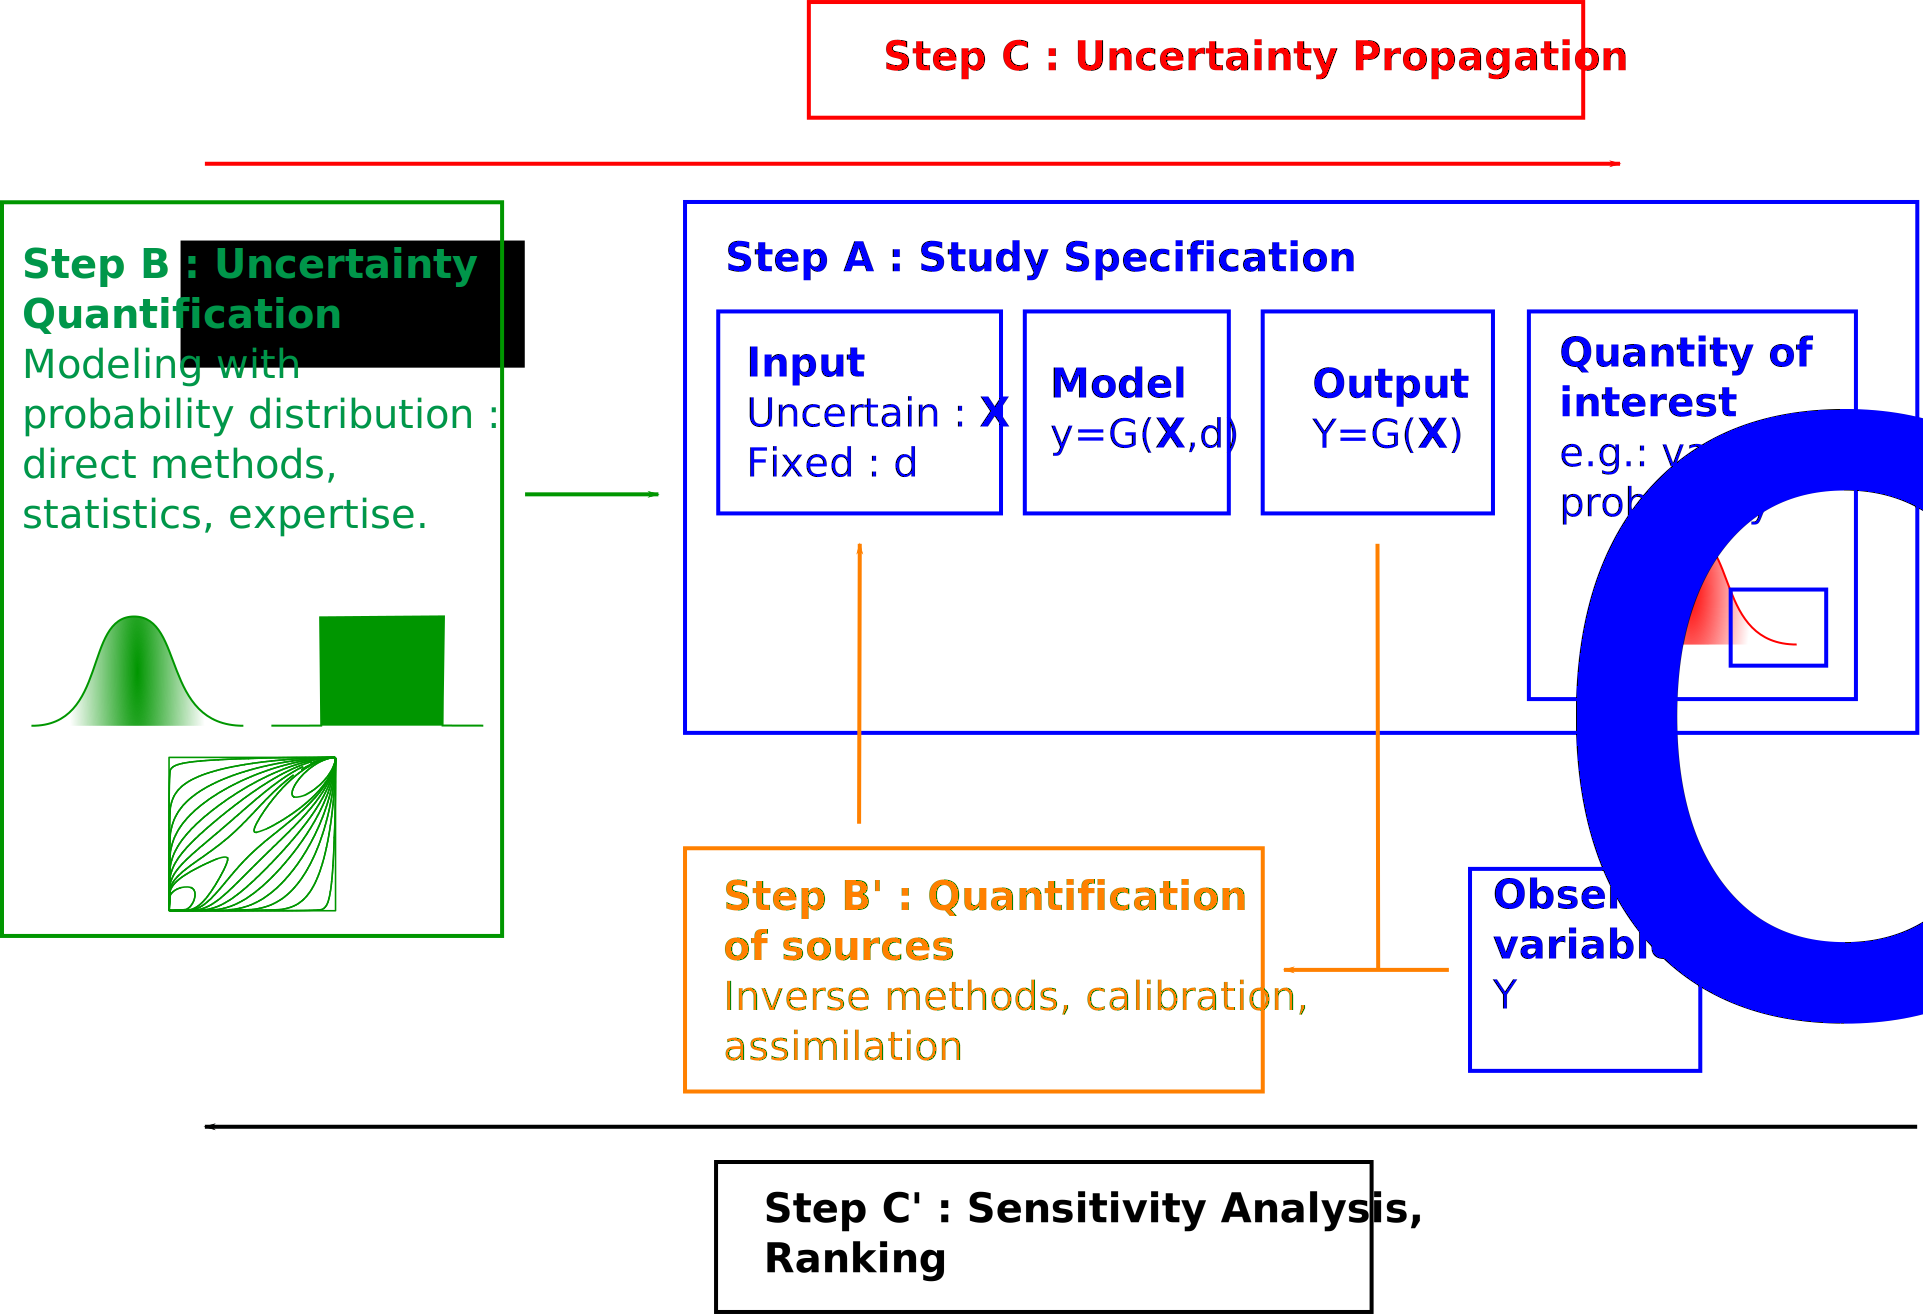
\includegraphics[width=0.9\textwidth]{figures/MethodologieIncertitude-EN}
\end{center}

\end{frame}


%%%%%%%%%%%%%%%%%%%%%%%%%%%%%%%%%%%%%%%%%%%%%%%%%%%%%%%%%%%%%%%%%%%%%%%%%%%%%
\section{The OpenTURNS library}

%%%%%%%%%%%%%%%%%%%%%%%%%%%%%%%%%%%%%%%%%%%%%%%%%%%%%%%%%%%%%%%%%%%%%%%%%%%%%

\begin{frame}
\frametitle{\ot{}}

  \begin{columns}
    \column{0.6\textwidth}
	
\begin{itemize}
\item Uncertainty quantification, uncertainty propagation, sensitivity analysis and metamodeling
\item Partners : EDF, Phiméca, Airbus, IMACS
\item \url{www.openturns.org}
\item Licence LGPL 
\item Linux, Windows
\end{itemize}

    \column{0.4\textwidth}

	\begin{center}
\includegraphics[width=0.9\textwidth]{figures/logo-ot}
\end{center}

	\end{columns}
\end{frame}

%%%%%%%%%%%%%%%%%%%%%%%%%%%%%%%%%%%%%%%%%%%%%%%%%%%%%%%%%%%%%%%%%%%%%%%%%%%%%

\begin{frame}[containsverbatim]
\frametitle{\ot{}}

  \begin{columns}
    \column{0.5\textwidth}
	
Fonctionnalités
\begin{itemize}
\item {\bf Étapes A, B, C, C'}
\item {\bf Processus stochastiques}
\item Méta-modèles : Chaos polynomial, Krigeage, Support Vector Machine
\item Estimation de probabilité de dépassement : 
FORM/SORM, Subset Sampling, Simulation Directionnelle Adaptative
\end{itemize}

    \column{0.5\textwidth}

Code de calcul G :
\begin{itemize}
\item Évaluation performante (multi-coeur) d'une formule analytique (avec calcul du 
gradient par dérivation symbolique)
\item Évaluation distribuée et multi-coeur d'une fonction Python (avec calcul du gradient 
par différences finies)
\item Par utilisation de la plate-forme SALOME
\end{itemize}

	\end{columns}

\end{frame}

%%%%%%%%%%%%%%%%%%%%%%%%%%%%%%%%%%%%%%%%%%%%%%%%%%%%%%%%%%%%%%%%%%%%%%%%%%%%%

\begin{frame}[containsverbatim]

Contexte :
  \begin{columns}
    \column{0.5\textwidth}
\frametitle{\ot{}}
\begin{itemize}
\item First release: 2007
\item 4 full time developpers
\item Users: mainly in France
\item Number of users: $\approx 1000$ (10900 Conda downloads in 2016-2017)
\end{itemize}

    \column{0.5\textwidth}

\frametitle{\ot{}}
\begin{itemize}
\item Taille du projet (2013) : 3600 fichiers, 550 classes, 250 000 lignes de code, 
1500 pages de documentation
\item Documentation : pour l'utilisateur du module Python, pour le développeur
\item Formations Itech : formation en 3 jours, 
\url{chercheurs.edf.com} : formation Itech "Incertitudes - Module 2"
\item TODO : Formation Phiméca ?
\end{itemize}

	\end{columns}

\end{frame}

%%%%%%%%%%%%%%%%%%%%%%%%%%%%%%%%%%%%%%%%%%%%%%%%%%%%%%%%%%%%%%%%%%%%%%%%%%%%%
\section{Diffusion d'OpenTURNS à EDF}

\begin{frame}[containsverbatim]
\frametitle{Contexte : des utilisations très variées}

  \begin{columns}
    \column{0.5\textwidth}
EDF
\begin{itemize}
\item Codes : physique des champs (code EF mécanique, CFD, thermique, ...), modèles 0D-1D, ...
\item Systèmes d'exploitation : Linux, Windows
\item Cartographie des utilisateurs : ingénieur d'étude non familier des méthodologies, chercheur non spécialiste, chercheur de l'équipe Incertitudes... 
\end{itemize}

    \column{0.5\textwidth}
\emph{Height of the river Garonne from Tonneins to La Réole (France), averaged over
70 000 random simulations of TELEMAC2D}
\begin{center}
\includegraphics[width=\textwidth]{figures/Garonne-Height-Mean}
\end{center}

  \end{columns}

\end{frame}

%%%%%%%%%%%%%%%%%%%%%%%%%%%%%%%%%%%%%%%%%%%%%%%%%%%%%%%%%%%%%%%%%%%%%%%%%%%%%

\section{Example}

\begin{frame}[containsverbatim]
\frametitle{Flood example 1/2}
\begin{adjustbox}{max width=\linewidth, margin=0pt}
\begin{lstlisting}[language=Python,basicstyle=\ttfamily,keywordstyle=\color{red}]
import openturns as ot
Q = ot.Gumbel(1./558., 1013.)
Ks = ot.Normal(30.0, 7.5)
Zv = ot.Uniform(49.0, 51.0)
Zm = ot.Uniform(54.0, 56.0)
dist = ot.ComposedDistribution([Q, Ks, Zv, Zm])
model = ot.SymbolicFunction(['Q', 'Ks', 'Zv', 'Zm'],
  ['(Q/(Ks*300.*sqrt((Zm-Zv)/5000)))^(3.0/5.0)+Zv-55.5-3.'])
rv = ot.RandomVector(dist)
\end{lstlisting}
\end{adjustbox}
\end{frame}

\begin{frame}[containsverbatim]
\frametitle{Flood example 2/2}

  \begin{columns}
    \column{0.6\textwidth}

\begin{adjustbox}{max width=\linewidth, margin=0pt}
\begin{lstlisting}[language=Python,basicstyle=\ttfamily,keywordstyle=\color{red}]
G = ot.CompositeRandomVector(model, rv)
event = ot.Event(G, ot.Greater(), 30.0)

optimAlgo = ot.Cobyla()
algo = ot.FORM(optimAlgo, event, dist.getMean())
algo.run()
result = algo.getResult()
print('Pf=', probability)
> Pf= 0.00670980426490075

result.drawImportanceFactors()
\end{lstlisting}
\end{adjustbox}
\column{0.4\textwidth}


\includegraphics[width=1.2\textwidth]{figures/imp_fact}

\end{columns}

\end{frame}

%%%%%%%%%%%%%%%%%%%%%%%%%%%%%%%%%%%%%%%%%%%%%%%%%%%%%%%%%%%%%%%%%%%%%%%%%%%%%

\section{Software architecture}

\begin{frame}[containsverbatim]

\begin{itemize}
\item C++ core / SWIG Python bindings
\item LAPACK / LibXml2 / TBB / muParser / NLopt
\item Packaging: Debian, Conda, Windows
\item Compilation: cmake
\item Documentation: Sphinx
\item Repository: https://github.com/openturns
\end{itemize}

\end{frame}

%%%%%%%%%%%%%%%%%%%%%%%%%%%%%%%%%%%%%%%%%%%%%%%%%%%%%%%%%%%%%%%%%%%%%%%%%%%%%

\section{Modules}

\begin{frame}[containsverbatim]
\frametitle{Modules}

\begin{itemize}
\item otrobopt: Robust optimization module

\item otfmi: FMI models manipulation

\item otsvm: SVM classifiers, metamodels

\item otagrum: Bayesian networks module

\item otwrapy: wrap external simulation codes

\item ...
\end{itemize}

\end{frame}

% %%%%%%%%%%%%%%%%%%%%%%%%%%%%%%%%%%%%%%%%%%%%%%%%%%%%%%%%%%%%%%%%%%%%%%%%%%%%%
% 
% \section{Features in development}
% 
% \begin{frame}[containsverbatim]
% \frametitle{Features in development}
% 
% \begin{itemize}
% \item Graphical User Interface (within SALOME)
% 
% \item Uncertainty quantification within 0D/1D models (Modelica) : 
% new partners on this topic are welcome !
% 
% \item Advanced vizualisation : functionnal data
% \end{itemize}
% 
% \end{frame}
%%%%%%%%%%%%%%%%%%%%%%%%%%%%%%%%%%%%%%%%%%%%%%%%%%%%%%%%%%%%%%%%%%%%%%%%%%%%%

\section{}

\begin{frame}
\frametitle{Bibliography}

\begin{itemize}
\item Airbus, EDF, Phimeca Engineering, IMACS. 
OpenTURNS, a scientific library usable as a Python module dedicated to the treatment of uncertainties, 
\url{www.openturns.org}.
\item Airbus, EDF, Phimeca Engineering, IMACS. Documentation of OpenTURNS, version 1.9. 
\url{http://openturns.github.io/openturns/1.9/contents.html}
\item  Michaël Baudin, Anne Dutfoy, Bertrand Iooss, and Anne-Laure Popelin. 
OpenTURNS: An Industrial Software for Uncertainty Quantification in Simulation, 
Handbook of Uncertainty Quantification, 
pages 1-38. Springer International Publishing, 2016
\item Open TELEMAC-MASCARET. 
Electricité de france, Sogreah, Hydraulic Research Wallingford, 
Centre d'Etudes Techniques Maritimes et Fluviales, Bundesanstalt fur Wasserbau, and Daresbury Laboratory.
\url{www.opentelemac.org}.
\end{itemize}

\end{frame}

%%%%%%%%%%%%%%%%%%%%%%%%%%%%%%%%%%%%%%%%%%%%%%%%%%%%%%%%%%%%%%%%%%%%%%%%%%%%%

%%%%%%%%%%%%%%%%%%%%%%%%%%%%%%%%%%%%%%%%%%%%%%%%%%%%%%%%%%%%%%%%%%%%%%%%%%%%%

\begin{frame}
\frametitle{END}

Thank you for your attention!

Any questions?

\begin{center}
\includegraphics[width=0.2\textwidth]{figures/logo-ot-small}
\end{center}

\end{frame}

\end{document}
